\chapter{Technical Design}\label{chap:technicaldesign}

Building on the goals, constraints, and use cases defined earlier, this chapter presents the system's technical foundation, focusing on data flow and the structure of core functionality. It begins with an overview of the client-server architecture and the division of responsibilities between frontend and backend. A sequence diagram illustrates how map data is retrieved and processed. The chapter then covers the client side, including how user interactions trigger updates and how the map is rendered. It also highlights the logic for classifying forestry roads based on environmental data. Finally, the server-side design is described, showing how the backend aggregates data, serves it to the frontend, and proxies external services.


\section{System Architecture}\label{sec:systemarchitecture}

The system follows a client-server architecture, where the website acts as a client and communicates with a backend server via a \acrshort{rest}ful \acrshort{api}. The processing of meteorological and geological data is handled on the server side, whereas frontend is responsible for requesting data, rendering maps, and presenting relevant information to the user. A simplified diagram of the system architecture is shown in \autoref{fig:systemarchitecture}.

\begin{figure}[h]
    \centering
    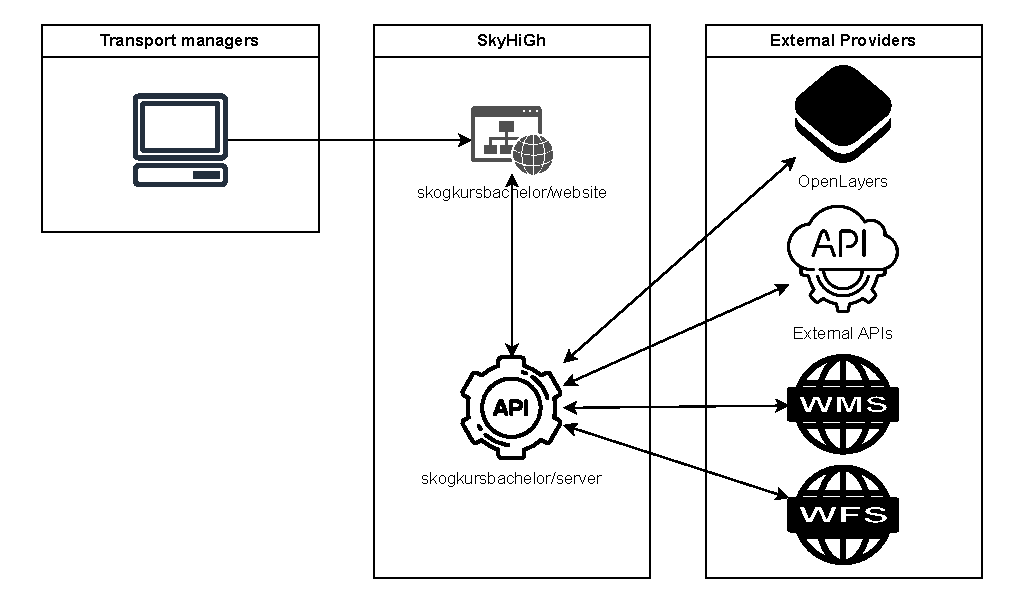
\includegraphics[width=1\linewidth]{figures/systemdesign.pdf}
    \caption{Schematic system architecture}
    \label{fig:systemarchitecture}
\end{figure}

The interaction between the website and the server is stateless, meaning that each request is independent and contains all the information needed to process it. This architectural choice improves system robustness and simplifies both development and deployment, particularly when it comes to scaling.

Additionally, the website is designed to only communicate with the outside world through the backend server. This decision, implemented using proxies and \acrshort{api} routes on the server, led to a cleaner and more maintainable architecture by centralizing all external communication through a single point.

\section{Sequence Diagram}

\begin{figure}[h]
    \centering
    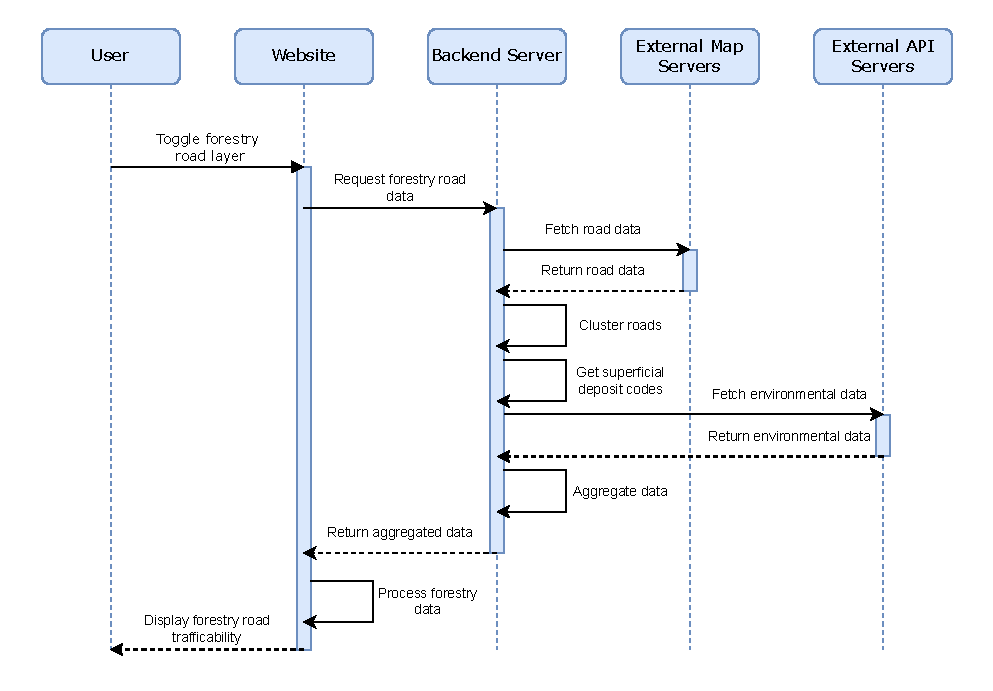
\includegraphics[width=1\linewidth]{figures/sequence_diagram.pdf}
    \caption{Sequence diagram of forestry road map layer}
    \label{fig:sequence_diagram}
\end{figure}

A sequence diagram illustrates how components interact over time to carry out an operation. It emphasizes the order of interactions between objects \cite{sequencediagram}. \autoref{fig:sequence_diagram} shows the interaction when the user toggles the forestry road map layer, which unfolds through the following steps:

\begin{enumerate}
    \item \textbf{Toggle forestry road layer}: The user toggles the forestry road map layer on the website.
    \item \textbf{Request forestry road data}: The website sends a request to the backend server for the necessary data within the visible map area.
    \item \textbf{Fetch road data}: The backend server fetches the required road data from an external \gls{wfs} server.
    \item \textbf{Return road data}: The map server return the requested road data.
    \item \textbf{Cluster roads:} The backend server clusters the roads into \qty{1}{\kilo\meter\squared} clusters.
    \item \textbf{Get superficial deposit codes:} The backend server queries for superficial deposits along all roads.
    \item \textbf{Fetch environmental data}: The backend server fetches environmental data for all clusters from an external \acrshort{api} server.
    \item \textbf{Return environmental data}: The external \acrshort{api} server returns environmental data.
    \item \textbf{Aggregate data}: The backend server aggregates all data into a single payload.
    \item \textbf{Return aggregated data}: The backend server sends the aggregated data back to the website.
    \item \textbf{Process forestry data}: The website processes the data and determines the trafficability of roads within the visible map area.
    \item \textbf{Display forestry road trafficability}: The forestry road layer, including trafficability, is rendered on the user's map.
\end{enumerate}

\section{Client-Side}\label{sec:technicaldesign:website}

The website serves as the user interface of the system, allowing users to visualize and interact with data related to forestry road conditions and weather-based forecasts using a dynamic map.

The classification of road trafficability is performed on the client side, as the website allows users to dynamically adjust thresholds for certain meteorological and geological parameters. A diagram detailing the classification is shown in \autoref{fig:forestryroadclassification}. Normally, this would be handled entirely by the backend server, but in order to provide immediate feedback when the user changes these thresholds, the classification logic is implemented in the frontend. This hybrid approach ensures a responsive user experience while keeping the most computationally expensive operations on the server.

\begin{figure}[h]
    \centering
    \centerline{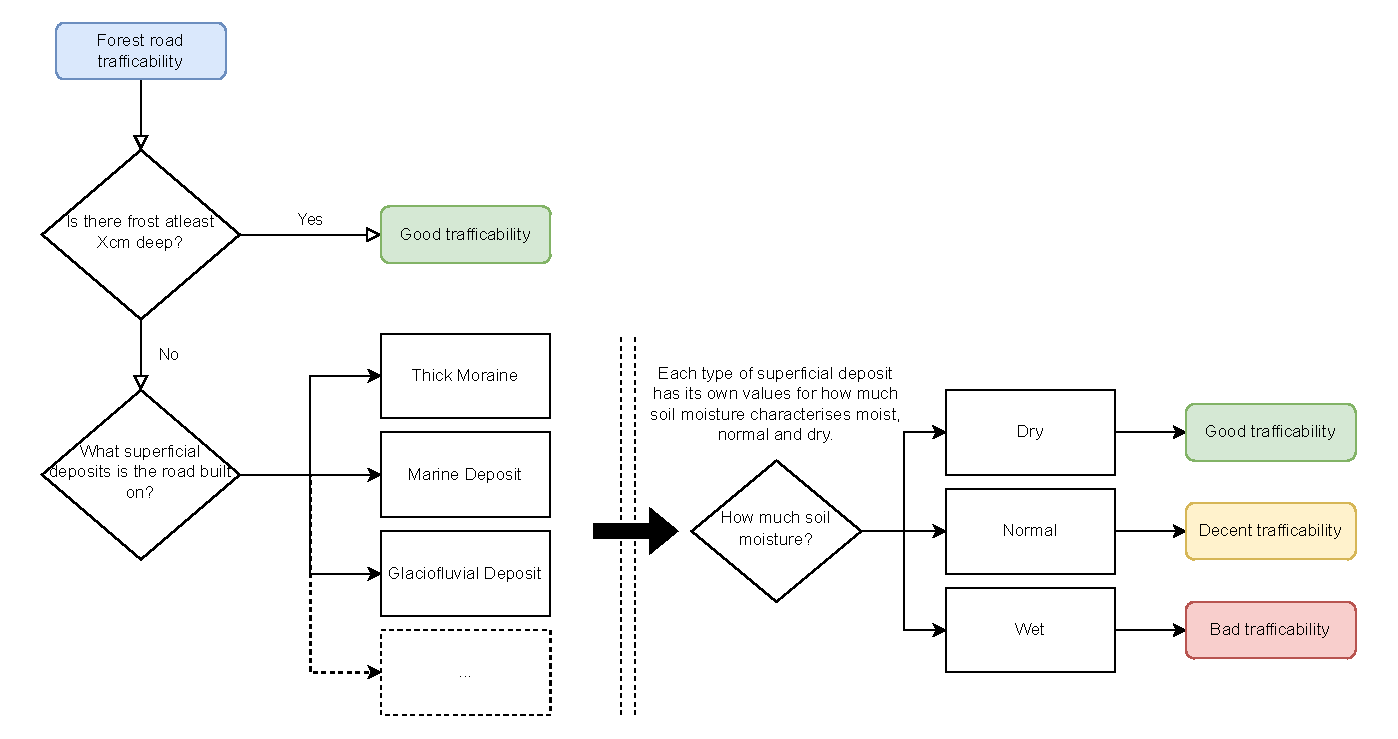
\includegraphics[width=1.2\linewidth]{figures/roadclassification.pdf}}
    \caption{Diagram visualizing the forestry road classification}
    \label{fig:forestryroadclassification}
\end{figure}

A central component of the website is its interactive map interface, which displays spatial data such as forestry road networks, map layers, and calculated trafficability classifications. The map is rendered dynamically in the browser using client-side resources, and data is loaded based on the user's current viewport and zoom level. This approach ensures more efficient data usage and better performance compared to loading the entire dataset at once.

The website is implemented as a single-page application (SPA), where all rendering and interface updates occur dynamically without full page reloads. This enables smooth interaction and better performance, as only relevant parts of the page are updated via the Document Object Model (DOM). \acrshort{html} 5 is required for full functionality, and the system relies on an active internet connection to fetch data from the server and external services. While the system is primarily intended for desktop and laptop use, it also runs on mobile devices, though the \acrshort{ui} is not optimized for smaller screens.

Choosing to implement the frontend as a web application provides several benefits. It ensures accessibility across a wide range of devices without the need for local installation, making the tool usable for different office environments.

Overall, the design of the website emphasizes a clean separation of concerns, efficiency in data handling, and accessibility, which together form a robust and user-friendly frontend component for the system.

% Backend Server, Backend Server ..., Server Design, Server Architecture
\section{Server-Side}

The server serves as the source of information for the website, providing map data for the website to visualize. This includes aggregation of different map data sources to create the forestry road layer, as well as forwarding \gls{wms} to the website.

As described above, the road classification is performed on the client side, and not in the backend server. This was done to decrease the amount of requests handled by the server, as the requests are aggregating data from multiple different sources, making them computationally expensive. As visualized in \autoref{fig:serverarchitecture}, the forestry roads endpoint fetches forestry road data for the from both an \acrshort{api} and \acrshort{wfs} server, in addition to local superficial deposit data.

\begin{figure}[h]
    \centering
    \centerline{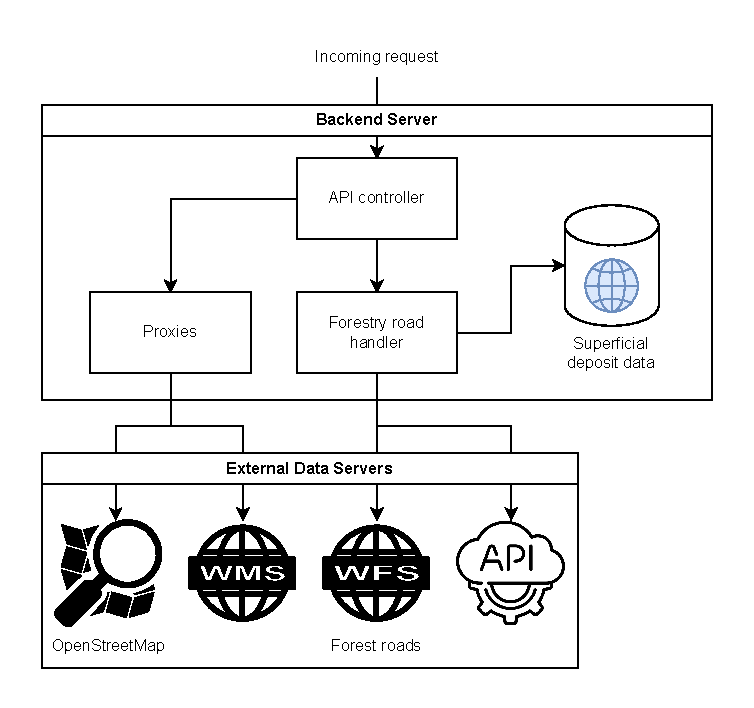
\includegraphics[width=1\linewidth]{figures/server.pdf}}
    \caption{Schematic diagram of backend server architecture}
    \label{fig:serverarchitecture}
\end{figure}

As briefly mentioned in \autoref{sec:systemarchitecture}, the server is designed as a \acrshort{rest}ful\footnote{\url{https://ics.uci.edu/~fielding/pubs/dissertation/rest_arch_style.htm}} \acrshort{api}. \acrfull{rest} is a software architectural style that defines a set of constraints for how the architecture of a distributed hypermedia system should behave, and is designed specifically for client-server applications. It emphasizes statelessness, caching, and layered systems \cite{restwiki}. 

Two of these constrains are specifically relevant to the design of the backend server. Statelessness is employed in the system, making each request contain as much information that is needed to fulfill it. This simplifies server logic and scalability, as the backend server does not need to store information between requests. The backend server is a layered system as it designed to be both an intermediary and the source, as there are proxies in addition to the forestry roads endpoint (see \autoref{fig:serverarchitecture}).

Using the server as an intermediary offers several advantages. While not all of these are utilized in this implementation, such an architecture allows for future expansion to include access control, credential protection for external services, and data filtering or transformation. It also simplifies integration with diverse external APIs by enabling consistent formatting before the data reaches the website.
